% figure1_propA.tex — Proposal A: single rich panel showing the full
% offload-repair loop. Top lane: agentic event sequence. Middle: GPU active
% KV cache (pale-blue). Bottom: Host buffer (dashed orange group).
% Two prominent arrows between middle and bottom: evict (down, dashed) and
% RepairKV (up, bold teal) carrying K teal rows. Signal s enters RepairKV.
% Shared preamble for standalone Figure 1 variants.
\documentclass[border=8pt,tikz]{standalone}
\usepackage{amsmath}
\usepackage{amssymb}
\usepackage{tikz}
\usetikzlibrary{arrows.meta,positioning,calc,fit,shapes.geometric,backgrounds}
\usepackage{xcolor}
\usepackage[T1]{fontenc}
\usepackage{mathptmx}
\newcommand{\repairkv}{\textsc{RepairKV}}
\newcommand{\bbase}{\ensuremath{B_{\mathrm{base}}}}
\newcommand{\bmatch}{\ensuremath{B_{\mathrm{match}}}}

\begin{document}
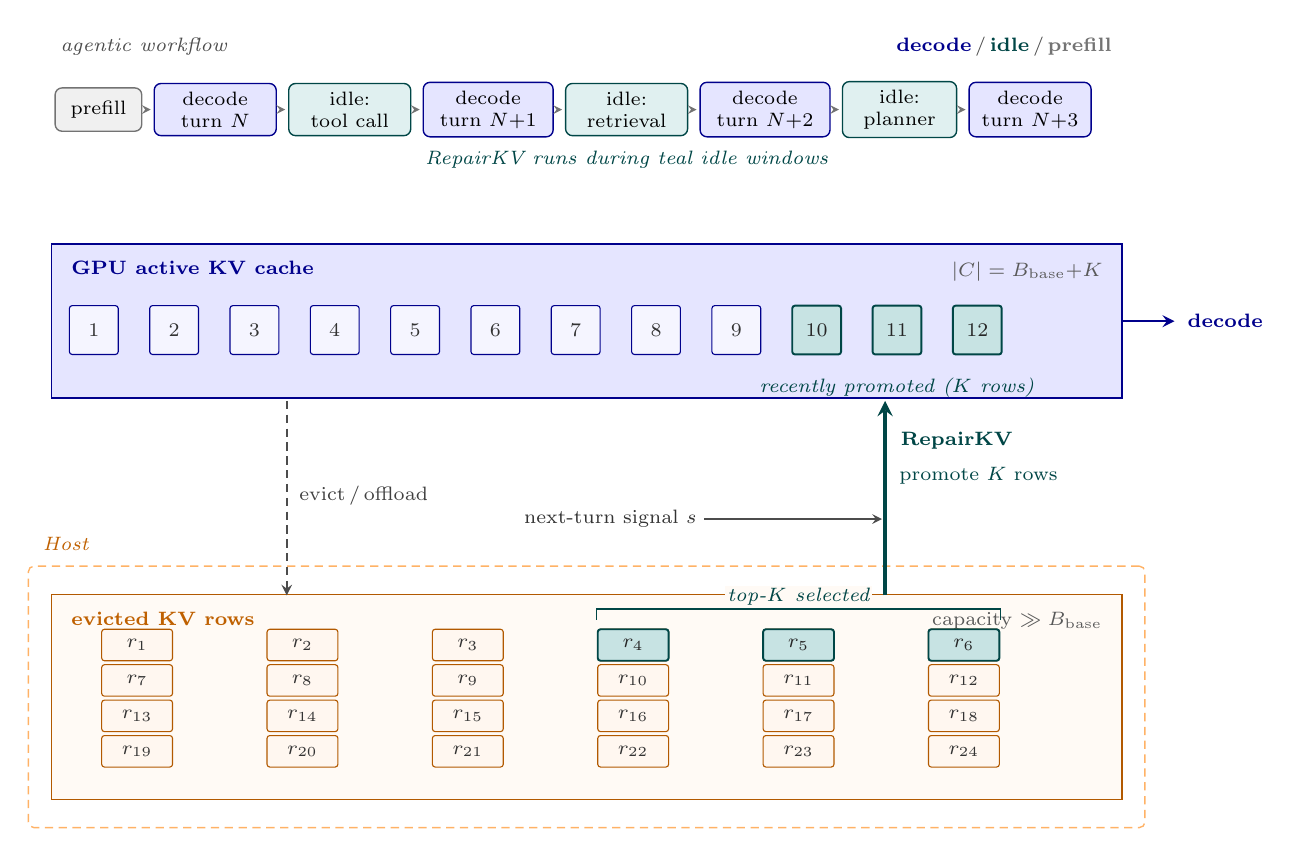
\begin{tikzpicture}[
  >=latex, line width=0.4pt,
  font=\small,
  % Generic block / panel rectangles
  panel/.style={draw=black, fill=white, line width=0.5pt,
                inner sep=6pt, align=center},
  active/.style={panel, fill=blue!10, draw=blue!55!black, line width=0.7pt},
  % Agentic-lane event pills
  evpill/.style={draw=black, line width=0.5pt, rounded corners=2.5pt,
                 inner sep=3pt, minimum height=0.55cm,
                 font=\scriptsize, align=center, fill=white},
  evdecode/.style={evpill, fill=blue!10,  draw=blue!55!black},
  evidle/.style  ={evpill, fill=teal!12,  draw=teal!55!black},
  evprefill/.style={evpill, fill=black!6, draw=black!55},
  laneconn/.style={->, line width=0.4pt, draw=black!55, >=stealth,
                   shorten >=1pt, shorten <=1pt},
  % KV slot tiles (numbered)
  slot/.style={draw=black!55, fill=white, line width=0.4pt,
               rounded corners=1pt, inner sep=0pt,
               minimum width=0.62cm, minimum height=0.62cm,
               font=\scriptsize, text=black!80},
  gpuslot/.style ={slot, draw=blue!55!black,  fill=blue!4},
  hostslot/.style={slot, draw=orange!70!black, fill=orange!6},
  promslot/.style={slot, draw=teal!55!black,  fill=teal!22, line width=0.7pt,
                   text=black!85},
  % Arrows
  arr/.style={->, line width=0.55pt, draw=black, >=stealth},
  evictarr/.style={->, line width=0.7pt, draw=black!70, dashed, >=stealth,
                   dash pattern=on 3pt off 2pt},
  repairarr/.style={->, line width=1.4pt, draw=teal!55!black, >=stealth},
  signalarr/.style={->, line width=0.55pt, draw=black!70, >=stealth},
  decodearr/.style={->, line width=0.9pt, draw=blue!55!black, >=stealth},
  % Labels
  arrlabel/.style={font=\scriptsize, text=black!75, fill=white, inner sep=1.5pt},
  arrlabelteal/.style={font=\scriptsize\bfseries, text=teal!55!black,
                       fill=white, inner sep=1.5pt},
  groupbox/.style={draw=orange!60, dashed, line width=0.5pt, rounded corners=2pt,
                   dash pattern=on 3pt off 2pt},
  grouplabel/.style={font=\scriptsize\itshape, text=orange!75!black},
  rowlabel/.style={font=\scriptsize\itshape, text=black!70},
  legendsmall/.style={font=\scriptsize, text=black!70}
]

% =========================================================================
% Frame coordinates
%   x: 0.4 .. 14.0   (panel width 13.6cm)
%   y bands:
%     top lane         ~ y = 5.30 .. 6.20
%     GPU panel        ~ y = 2.10 .. 4.05  (height 1.95cm)
%     vertical arrows  ~ y = -0.40 .. 2.10
%     Host panel       ~ y = -3.00 .. -0.40 (height 2.60cm)
%     dashed Host group sits ~ 0.30cm beyond host panel
% =========================================================================

\def\xL{0.4}
\def\xR{14.0}
\def\panelW{13.6cm}

% =========================================================================
% TOP LANE: agentic workflow (8 events)
% =========================================================================
\node[rowlabel, anchor=west] at (\xL, 6.55) {agentic workflow};
\node[legendsmall, anchor=east] at (\xR, 6.55)
  {{\color{blue!55!black}\textbf{decode}}\,/\,%
   {\color{teal!55!black}\textbf{idle}}\,/\,%
   {\color{black!55}\textbf{prefill}}};

\node[evprefill, minimum width=1.10cm, anchor=west] (e1) at (\xL+0.05, 5.75)
  {prefill};
\node[evdecode,  minimum width=1.55cm, right=4pt of e1] (e2)
  {decode\\turn $N$};
\node[evidle,    minimum width=1.55cm, right=4pt of e2] (e3)
  {idle:\\tool call};
\node[evdecode,  minimum width=1.65cm, right=4pt of e3] (e4)
  {decode\\turn $N{+}1$};
\node[evidle,    minimum width=1.55cm, right=4pt of e4] (e5)
  {idle:\\retrieval};
\node[evdecode,  minimum width=1.65cm, right=4pt of e5] (e6)
  {decode\\turn $N{+}2$};
\node[evidle,    minimum width=1.45cm, right=4pt of e6] (e7)
  {idle:\\planner};
\node[evdecode,  minimum width=1.55cm, right=4pt of e7] (e8)
  {decode\\turn $N{+}3$};

\foreach \a/\b in {e1/e2, e2/e3, e3/e4, e4/e5, e5/e6, e6/e7, e7/e8}{
  \draw[laneconn] (\a.east) -- (\b.west);
}

% =========================================================================
% MIDDLE: GPU active KV cache  (12 slots; rightmost 3 are teal/promoted)
% =========================================================================
\node[active, anchor=north west, minimum width=\panelW, minimum height=1.95cm]
  (gpu) at (\xL, 4.05) {};

% Header label inside the panel (top-left)
\node[font=\scriptsize\bfseries, text=blue!55!black, anchor=north west]
  at ([xshift=4pt, yshift=-3pt]gpu.north west) {GPU active KV cache};

% Capacity annotation top-right
\node[font=\scriptsize, text=black!65, anchor=north east]
  at ([xshift=-4pt, yshift=-3pt]gpu.north east) {$|C|=\bbase{+}K$};

% 12 numbered slots, evenly spaced
\foreach \i in {1,...,9}{
  \pgfmathsetmacro{\xc}{\xL + 0.55 + (\i-1)*1.02}
  \node[gpuslot] (g\i) at (\xc, 2.95) {\i};
}
\foreach \i in {10,11,12}{
  \pgfmathsetmacro{\xc}{\xL + 0.55 + (\i-1)*1.02}
  \node[promslot] (g\i) at (\xc, 2.95) {\i};
}

% Inline annotation BELOW the 3 teal slots, inside the GPU panel.
\node[font=\scriptsize\itshape, text=teal!55!black, anchor=north]
  at ($(g10.south)!0.5!(g12.south) + (0,-0.16)$)
  {recently promoted ($K$ rows)};

% =========================================================================
% BOTTOM: Host buffer (4 rows x 5 cols = 20 slots; 3 teal at top-right)
% =========================================================================
\node[panel, fill=orange!4, draw=orange!70!black, anchor=north west,
      minimum width=\panelW, minimum height=2.60cm]
  (host) at (\xL, -0.40) {};

% Header inside panel (top-left)
\node[font=\scriptsize\bfseries, text=orange!75!black, anchor=north west]
  at ([xshift=4pt, yshift=-3pt]host.north west) {evicted KV rows};

\node[font=\scriptsize, text=black!65, anchor=north east]
  at ([xshift=-4pt, yshift=-3pt]host.north east) {capacity $\gg \bbase$};

% 4 rows x 6 cols = 24 host entries (denser, more host-like)
% Inner area: x in [xL+0.5, xR-0.5] -> usable ~ 12.6, slot width 0.9cm
% Spacing: 6 slots over 12.6cm  -> step = 12.6/6 = 2.10
\foreach \r in {0,1,2,3}{
  \foreach \c in {1,...,6}{
    \pgfmathsetmacro{\xh}{\xL + 1.10 + (\c-1)*2.10}
    \pgfmathsetmacro{\yh}{-1.05 - \r*0.45}
    \pgfmathsetmacro{\idx}{int(\r*6+\c)}
    \node[hostslot, minimum width=0.9cm, minimum height=0.40cm]
         (h\r-\c) at (\xh, \yh) {\scriptsize $r_{\idx}$};
  }
}

% Recolor the 3 selected rows in the top row, columns 4,5,6 (right cluster)
\node[promslot, minimum width=0.9cm, minimum height=0.40cm]
  (sel1) at ($(h0-4)$) {\scriptsize $r_{4}$};
\node[promslot, minimum width=0.9cm, minimum height=0.40cm]
  (sel2) at ($(h0-5)$) {\scriptsize $r_{5}$};
\node[promslot, minimum width=0.9cm, minimum height=0.40cm]
  (sel3) at ($(h0-6)$) {\scriptsize $r_{6}$};

% Bracket ABOVE the 3 teal selected slots
\draw[teal!55!black, line width=0.5pt]
  ([yshift=3pt]sel1.north west) -- ([yshift=7pt]sel1.north west)
  -- ([yshift=7pt]sel3.north east) -- ([yshift=3pt]sel3.north east);
\node[font=\scriptsize\itshape, text=teal!55!black, anchor=south,
      fill=orange!4, inner sep=1pt]
  at ($([yshift=7pt]sel1.north west)!0.5!([yshift=7pt]sel3.north east)$)
  {top-$K$ selected};

% Dashed orange "Host" group around the host panel
\node[groupbox, fit=(host), inner xsep=8pt, inner ysep=10pt] (hgroup) {};
\node[grouplabel, anchor=south west]
  at ([xshift=2pt, yshift=2pt]hgroup.north west) {Host};

% =========================================================================
% TWO PROMINENT ARROWS BETWEEN GPU AND HOST
%   - Evict / offload: dashed, DOWN, on the LEFT  (x = 3.4)
%   - RepairKV:        bold teal, UP, on the RIGHT (x = 11.0)
% Vertical span: GPU bottom y=2.10 -> Host top y=-0.40
% =========================================================================

\def\xEvict{3.4}
\def\xRepair{11.0}

% Evict (down, dashed)
\draw[evictarr]
  (\xEvict, 2.05) -- (\xEvict, -0.42);
\node[arrlabel, anchor=west]
  at (\xEvict+0.10, 0.85) {evict\,/\,offload};

% RepairKV (up, bold teal)
\draw[repairarr]
  (\xRepair, -0.42) -- (\xRepair, 2.05);
\node[arrlabelteal, anchor=west]
  at (\xRepair+0.14, 1.55) {\repairkv{}};
\node[font=\scriptsize, text=teal!55!black, anchor=west, fill=white, inner sep=1pt]
  at (\xRepair+0.14, 1.10) {promote $K$ rows};

% --- Signal s entering the RepairKV arrow midpoint ---
% A SHORT arrow with the "next-turn signal s" label, entering from the LEFT
% horizontally onto the RepairKV shaft midpoint.
\coordinate (sTip)   at (\xRepair-0.04, 0.55);
\coordinate (sStart) at (\xRepair-2.30, 0.55);
\draw[signalarr] (sStart) -- (sTip);
\node[font=\scriptsize, text=black!80, anchor=east, fill=white, inner sep=1.5pt]
  at ([xshift=-1pt]sStart) {next-turn signal $s$};

% =========================================================================
% RIGHT EDGE: decode output exiting GPU
% =========================================================================
\draw[decodearr]
  (gpu.east) -- ++(0.65, 0)
  node[font=\scriptsize\bfseries, text=blue!55!black, anchor=west, xshift=1pt]
  {decode};

% =========================================================================
% Subtle band-label between top lane and GPU
% =========================================================================
\node[font=\scriptsize\itshape, text=teal!55!black, anchor=center]
  at ($(e5.south)+(0,-0.30)$) {RepairKV runs during teal idle windows};

\end{tikzpicture}
\end{document}
